\documentclass[14pt, a4paper]{report}
\usepackage{mathtext}
\usepackage[T2A]{fontenc}
\usepackage[utf8]{inputenc}
\usepackage[russian]{babel}
\usepackage{multirow}
\usepackage{slashbox}
\usepackage{makecell}
\usepackage{graphicx}
\usepackage{physics}
\usepackage{amstext}
\usepackage{caption}
\usepackage{subcaption}
\usepackage{cmap}
\usepackage{float}
\usepackage{indentfirst}

\usepackage[a4paper,
            		left=1in,
            		right=1in,
           		 top=1in,
            		bottom=1in,
            		footskip=.25in]{geometry}

\renewcommand{\thesection}{\arabic{section}.}
\renewcommand{\thesubsection}{\arabic{section}.\arabic{subsection}.}

\title{\textbf{Отчет о выполнении лабораторной работы 4.2 "Исследование энергетического спектра $\beta$-частиц и определение их максимальной энергии при помощи магнитного спектрометра"}}
\author{Калашников Михаил, Б03-202б}
\date{}

\begin{document}
\maketitle

\textbf{Цель работы:}
Исследовать с помощью магнитного спектрометра энергетический спектр $\beta$-частиц при распаде ядер $^{137}$Cs и определить их максимальную энергию. Откалибровать спектрометр по энергии электронов внутренней конверсии $^{137}$Cs.

\textbf{В работе используются:}
\begin{itemize}
\item магнитный спектрометр
\end{itemize}

\section{Теоретические сведения}

Бета-распадом называется самопроизвольное превращение ядер, при котором их массовое число остается прежним, а заряд изменяется на единицу. Бета-активные ядра встречаются во всей области значений массового числа A.
В данной работе будет изучен электронный распад
\[^A_Z X \rightarrow _{Z+1}^A X+e^-+\tilde{\nu},\]
при котором кроме электрона испускается антинейтрино.

Спектр энергии $\beta$-частиц оценивается формулой
\[\frac{dN}{dE}\approx\sqrt{E}(E_e-E)^2,\]
где $E_e$ -- максимальная энергия электронов.

Дочерние ядра, возникающие в результате $\beta$-распада, нередко оказываются возбужденными. Такие ядра отдают свою энергию либо излучая $\gamma$-квант, либо передевая избыток энергии одному из электронов с внутренних оболочек атома. Излучаемые в таком процессе электроны имеют строго определенную энергию и называются конверсионными.

\begin{figure}[H]
\centering
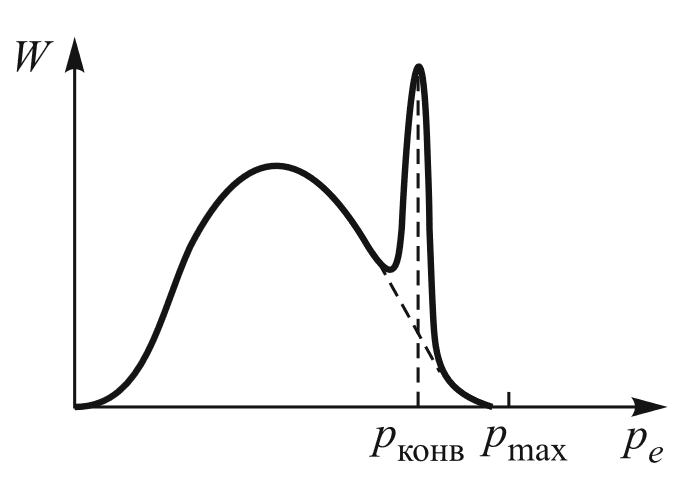
\includegraphics[scale=0.5]{../images/542-1}
\caption{Форма спектра $\beta$-частиц}
\end{figure}

\section{Экспериментальная установка}

Для определения энергии $\beta$-частиц используется магнитный $\beta$-спектрометр. Электроны, испускаемые радиоактивным источником попадают в магнитное поле катушки. Траектории электронов в магнитном поле являются сложной спиралью, сходящимися в фокусе. В фокусе установлен детектор электронов.

\section{Проведение эксперимента}

\section{Обработка результатов}

\section{Выводы}

\end{document}